\subsubsubsection{Пример: FFT удаление шума}
\\\\
\indent Основываясь на теореме (\myref{thm::parceval}), приводим в качестве примера решение задачи об удалении шума. К сожалению, в силу постоянства спектра сигнала, данные, исследуемые в блоке (\myref{link::mssa}) в качестве примера для сравнения использовать не получится, так как ключевой их особенностью является наличие трендовой составляющей. Следовательно с течение времени частота сигнала изменяется, однако предположив периодичность каждый $[-5, 5]$, получаем возможность приблизить на данном отрезке функцию. Следовательно, можем перейти в пространство частот для данного участка. То есть ничто не мешает технически вычислить коэффициенты Фурье и, основываясь на них, <<очистить>> исходную функцию от шума.
\begin{figure}[H]
	\centering
	\begin{tikzpicture}
		\begin{axis}[
			grid = both,
			legend pos = north west,
			minor tick num = 1,
			major grid style = {lightgray},
			minor grid style = {lightgray!25},
			%title= {},
			width = \textwidth,
			height = 0.45 \textwidth,
			xmin=-5, xmax=5,
			ymin=-4, ymax=7.5,
			line width=0.3mm
			]
			
			\addplot[color = orange, line width = 0.035cm] table [
			x=x, 
			y=y_clean, 
			col sep=comma,
			mark={},
			] {./source/source_csv/Illustration data/fft/denoised_data_incorrect.csv};
			
			\addplot[opacity = 0.25, color = blue] table [
			x=x, 
			y=y_initial, 
			col sep=comma,
			mark={},
			] {./source/source_csv/Illustration data/fft/denoised_data_incorrect.csv};
			
			\addplot[domain = -5:5,
			samples = 300,
			color = teal,
			smooth,
			line width = 0.025cm,] {sin(deg(5 * x)) + 1 / 4 * (x^2)};
			
			\legend{$f(x)$ очищенный, $f(x)$ c шумом, $f(x)$ без шума};
		\end{axis}
	\end{tikzpicture}
	\caption{Очистка ряда от шума посредством преобразования Фурье}
\end{figure}
Из графика видим, что восстановление прошло намного лучше, чем было изначально представлено в (\myref{link::mssa}), что обусловлено цикличностью данного отрезка, то есть спрогнозировать что-либо новое за пределами восстановленной области (дальше, чем $[-5, 5]$) не получится, так как все, что дальше - это повтор того, что находится на данном отрезке. Настоящий ряд, в котором отсутствует шум был восстановлен через  использование первых $8$-и частот, показавших наибольшие амплитуды.

Более того, график зависимости качества восстановления от количества использованных частот имеет вид:
\begin{figure}[H]
	\centering
	\begin{tikzpicture}
		\begin{axis}[
			grid = both,
			legend pos = north west,
			minor tick num = 1,
			major grid style = {lightgray},
			minor grid style = {lightgray!25},
			%title= {},
			width = \textwidth,
			height = 0.45 \textwidth,
			xmin=1, xmax=80,
			ymin=-4, ymax=7.5,
			line width=0.3mm
			]
			
			\addplot[line width = 0.035cm] table [
			x=k, 
			y=rmse, 
			col sep=comma,
			mark={},
			] {./source/source_csv/Illustration data/fft/statisticalDataRMSE.csv};
			\addplot +[mark=none] coordinates {(8, -4) (8, 8)};
			
			\node at (250,600) {$k = 8$, RMSE$(8) = 0.079$};
			
			\draw[->] (110,600) -- (75, 450);
			\legend{$k$ - количество использованных частот};
		\end{axis}
	\end{tikzpicture}
	\caption{RMSE$(k)$ - ошибка Root Mean Squared Error для восстановленного ряда относительно истинного ряда без шума. RMSE = $\sqrt{\text{MSE}} = \sqrt{1 / n \sum(\hat{y}_j - y_j)^2}$}
\end{figure}
Однако, несмотря на такой хороший результат, нельзя забывать, что 1) у преобразования Фурье существует гиперпараметр, отвечающий за количество используемых для восстановления частот 2) исходная функция (без шума) в реальности почти всегда не является наблюдаемой, то есть не от чего отталкиваться, чтобы измерить ошибку RMSE. А значит, на данный моменты в настоящей работе MSSA остается лидером в вопросе непараметризованной очистки данных от шума.

В качестве более удачного примера рассматриваем функцию вида:
\begin{equation} \label{link::new_function}
	f(t) = 1.25 \sin(3x) + 2\cos(4x) + 2.5 \cdot \varepsilon: \; \varepsilon \sim N(0, 1)
\end{equation}
Изначально график функции с уже примененным алгоритмом очистки путем преобразования Фурье имеет вид:
\begin{figure}[H]
	\centering
	\begin{tikzpicture}
		\begin{axis}[
			grid = both,
			legend pos = north west,
			minor tick num = 1,
			major grid style = {lightgray},
			minor grid style = {lightgray!25},
			%title= {},
			width = \textwidth,
			height = 0.45 \textwidth,
			xmin=-5, xmax=5,
			ymin=-10, ymax=10,
			line width=0.3mm
			]
			
			\addplot[opacity= 0.3, color= purple] table [
			x=x, 
			y=y_initial, 
			col sep=comma,
			mark={},
			] {./source/source_csv/Illustration data/fft/denoised_data_correct.csv};
			
			\addplot[domain = -5:5,
			samples = 300,
			color = teal,
			smooth,
			line width = 0.025cm,] {1.25 * sin(deg(3 * x)) + 2 * cos(deg(4 * x))};
			
			\addplot table [
			x=x, 
			y=y_clean, 
			col sep=comma,
			mark={},
			] {./source/source_csv/Illustration data/fft/denoised_data_correct.csv};
						

			\legend{$f(t)$ с шумом, $f(t)$ без шума, $f(t)$ очищенная};
		\end{axis}
	\end{tikzpicture}
	\caption{Построение функции $(\ref{link::new_function})$}
\end{figure}
В свое время график амплитуд, имеет вид:
\begin{figure}[H]
	\centering
	\begin{tikzpicture}
		\begin{axis}[
			grid = both,
			legend pos = north west,
			minor tick num = 1,
			major grid style = {lightgray},
			minor grid style = {lightgray!25},
			%title= {},
			width = \textwidth,
			height = 0.45 \textwidth,
			xmin=0, xmax=0.05,
			ymin=0, ymax=0.9,
			line width=0.3mm,
			xlabel= Частота,
			ylabel= Амплитуда
			]
			
			\addplot table [
			x=f, 
			y=power, 
			col sep=comma,
			mark={},
			] {./source/source_csv/Illustration data/fft/denoised_data_correct.csv};
			\addplot +[mark=none] coordinates {(0.025125628, 0) (0.025125628, 0.9)};
						
			\legend{Амплитуда};
		\end{axis}
	\end{tikzpicture}
	\caption{Построение спектра амплитуд функции (\ref{link::new_function})}
\end{figure}
Интересно, что данный график является симметричным относительно $f = 0.025$, поэтому часто используется половина данного графика \cite{brunton2022data}. Исходя из получившегося изображения, замечаем что существуют частоты наиболее сильно <<звучащие>> в сигнале, то есть они, скорее всего, являются именно звуком (трендом), а не шумом. То есть коэффициенты, соответствующие им, обнулять не нужно, в отличие от других, колеблющихся в пределах от $0.4$ до 0. Они, может быть, представляют из себя шум, то есть подлежат обнулению.

Таким образом, прямым назначением как алгоритма FFT, так и самого преобразования Фурье, в настоящей работе является очистка показателей от шумовой компоненты, а также - проведения гармонического анализа  (в большей части из-за требования стационарности амплитудного спектра для этого применяется Wavelet преобразование (\myref{link::wavelet_analysis})) доходностей акций или их цент, так как визуально данные показатели можно назвать сигналами. Соответственно выделив <<управляющую>> частоту, получаем тренд для цен, что позволяет далее более уверенно говорить об устойчивости финансовой позиции и минимизации риска портфеля некоторого рыночного агента.

Доказательством неприменимости самого преобразования Фурье для частотного анализа временных рядов служит визуальное представление графика доходностей компании Apple. Однако сами по себе графики цены открытия и доходности цены открытия мало что говорят о самой частоте, то есть о том, на чем специализируется гармонический анализ. Смотрим на графики цены и доходности, соотнося их с графиками собственных амплитуд:
\begin{figure}[H]
	\centering
	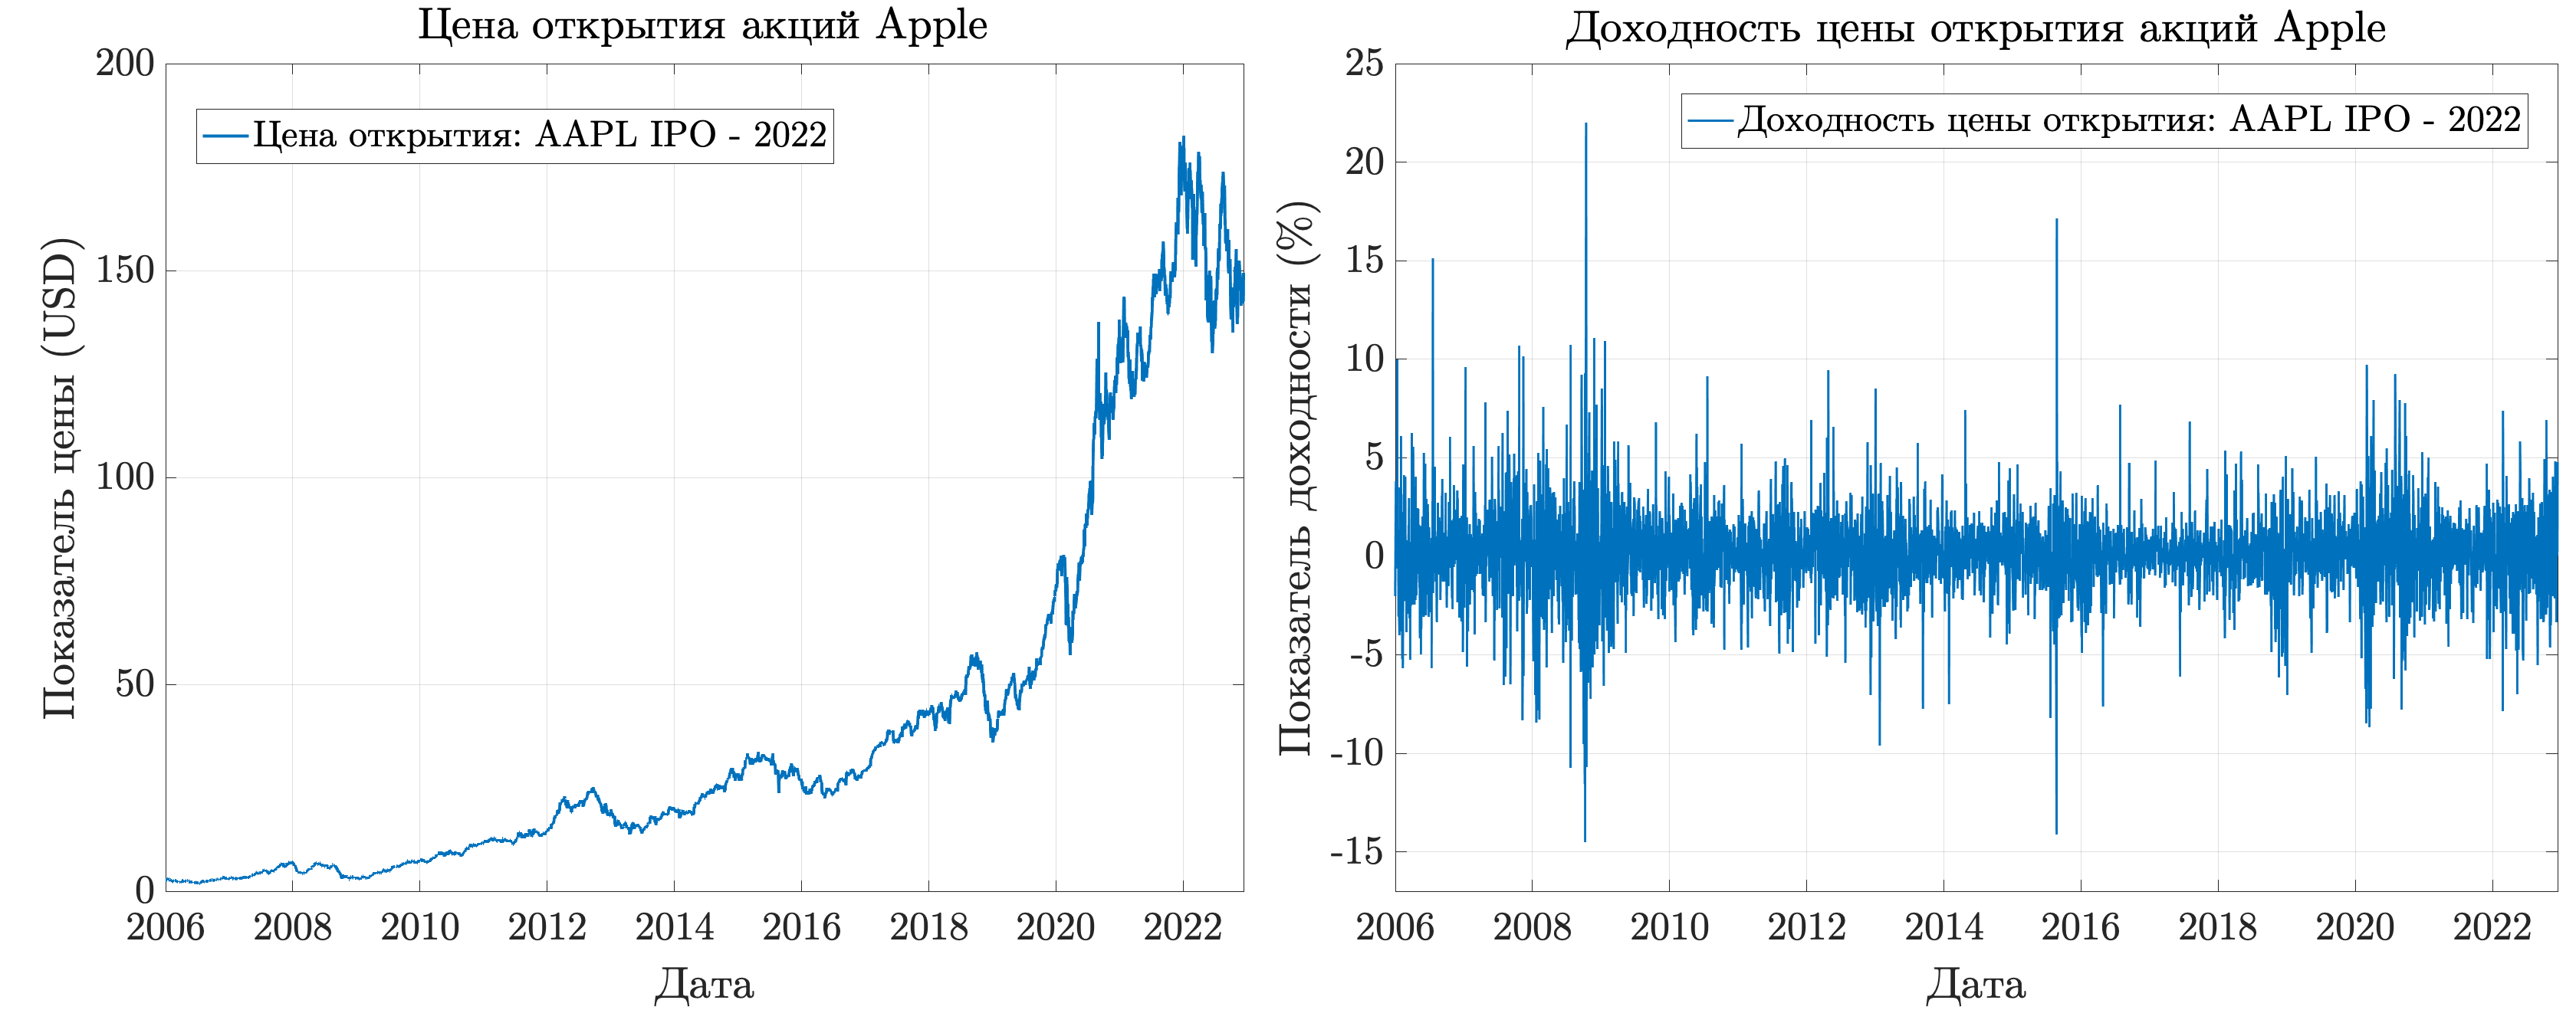
\includegraphics[width=17cm]{returns pictures/apple_prices_returns.png}
	\caption{График цены открытия и доходности Apple (IPO - 2022)}
	\label{fig::apple_prices_returns}
\end{figure}
\noindent А теперь графики амплитуд соответственно. Глядя на график (\ref{fig::amplitudes_apple_prices_returns}), видим, что показатель цены акции не содержит в себе значимой частотной информации, то есть выделить некоторые наиболее сильно <<звучащие>> частоты не удалось. Пик в самом начале (и симметричный ему в конце) отвечает за среднее значение, так как, подставляя в выражение (\myref{equation::fourier_approximation}) $k = 0$, получаем константу. Однако, исходя из амплитуд доходности, понимаем, что они, в свою очередь, включают в себя достаточно большое количество информации о частотах. Но пока что это еще не успех, так как, основываясь на том же графике (\ref{fig::amplitudes_apple_prices_returns}), получается, что значимы все частоты. 
\begin{figure}[H]
	\centering
	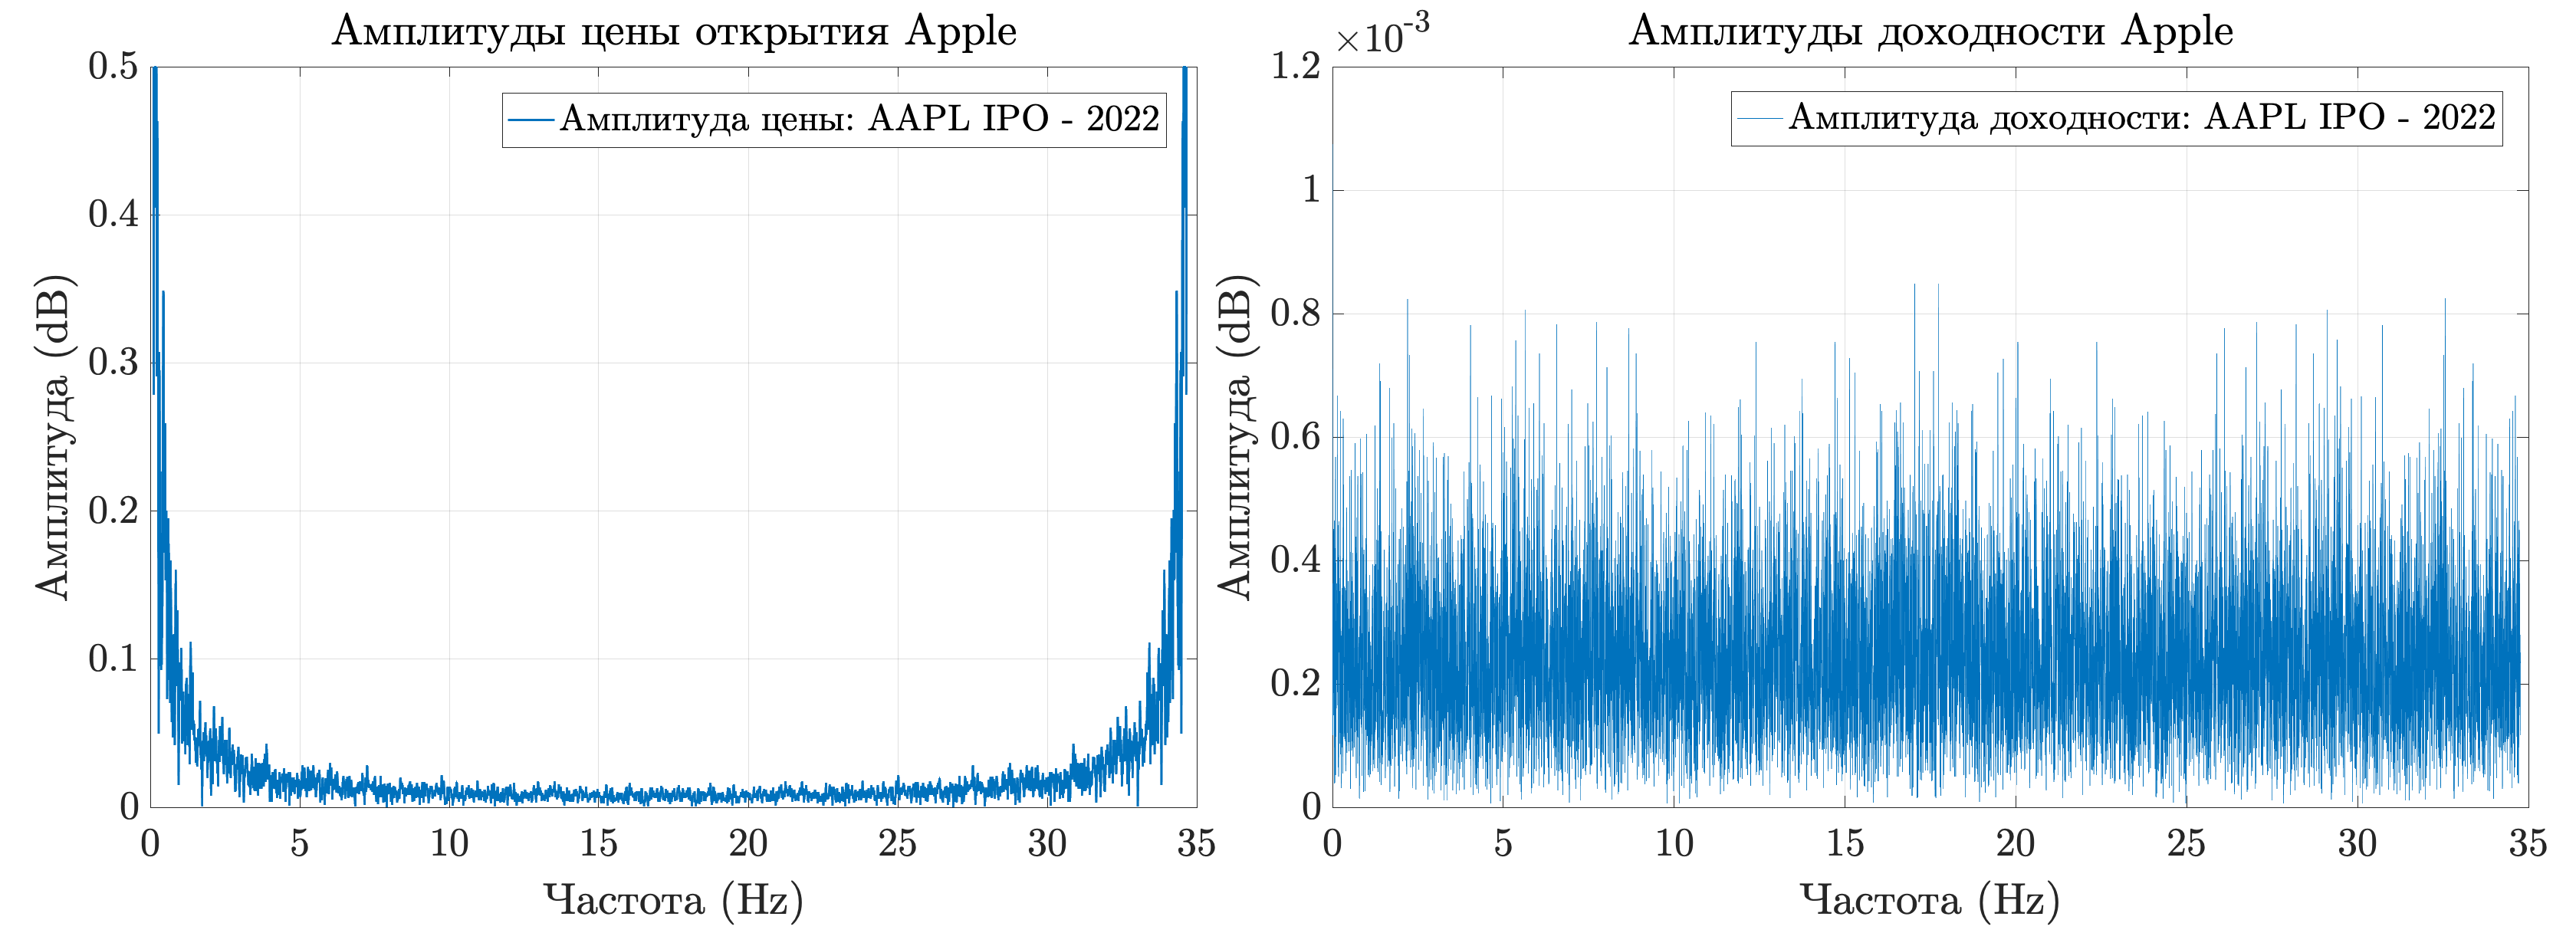
\includegraphics[width=17cm]{time frequency/amplitudes_apple_prices_returns.png}
	\caption{График амплитуд цены открытия и доходности Apple (IPO - 2022)}
	\label{fig::amplitudes_apple_prices_returns}
\end{figure}
Глядя же на график (\ref{fig::apple_prices_returns}) очевидно, что в <<сигнале>> доходности частота разная для каждого периода времени. Это характеризуется разной степенью волатильности показателя доходности, как уже отмечалось в (\myref{link::garch_block}), а также (\myref{link::figarch}). Иными словами, ранее говорилось об <<условной гетероскедастичности>>, а теперь говорится о <<непостоянстве частот во времени>>.

Таким образом, получается, что анализ Фурье применим к анализу финансовых рядов (в особенности доходностей), однако, исходя из самих значений сигнала, нарушается главная предпосылка - постоянство частот во времени. Следовательно, необходим подход, основанный на анализе Фурье, но учитывающий при это непостоянство частот. Это и есть Wavelet анализ (см. \myref{link::wavelet_analysis}), речь о котором идет далее.